\documentclass[a4paper, 12pt, final, garamond]{book}
\usepackage{cours-preambule}

\raggedbottom

\makeatletter
\renewcommand{\@chapapp}{Programme de kh\^olle -- semaine}
\makeatother

\begin{document}
\setcounter{chapter}{16}

\chapter{Du 30 janvier au 03 f\'evrier}

\section{Cours et exercices}
\section*{Mécanique chapitre 2 -- Dynamique du point}
\begin{enumerate}[label=\Roman*]
    \item \textbf{Introduction}~: inertie et quantité de mouvement, forces
        fondamentales.
    \item \textbf{Trois lois de \textsc{Newton}}~: principe d'inertie, principe
        fondamental de la mécanique, loi des actions réciproques.
    \item \textbf{Systèmes de points}~: centre d'inertie, quantité de mouvement
        d'un ensemble de points, théorème de la résultante cinétique.
    \item \textbf{Méthode générale de résolution}.
    \item \textbf{Le poids}~: définition, chute libre avec angle initial.
    \item \textbf{Poussée d'\textsc{Archimède}}.
    \item \textbf{Frottement fluide}~: force de frottement fluide, chute libre
        sans vitesse initiale avec frottements linéaires, avec frottements
        quadratique, résolution par adimensionnement.
    \item \textbf{Frottements solides}~: réaction, lois de \textsc{Coulomb}.
    \item \textbf{Tension d'un fil}
    \item \textbf{Force de rappel d'un ressort}~: force de rappel élastique,
        position d'équilibre verticale.
\end{enumerate}

\section*{Mécanique chapitre 3 -- Mécanique des mouvements courbes}
\begin{enumerate}[label=\Roman*]
    \item \textbf{Mouvement courbe dans le plan}~: position, vitesse,
        déplacement élémentaire, accélération en coordonnées polaires.
    \item \textbf{Exemples de mouvements plans}~: mouvement circulaire,
        circulaire uniforme, repère de \textsc{Frenet}.
    \item \textbf{Application~: pendule simple}
    \item \textbf{Mouvement courbe dans l'espace}~: coordonnées cylindriques,
        coordonnées sphériques.
\end{enumerate}

\section{Cours uniquement}
\section*{Mécanique chapitre 4 -- Approche énergétique}
\begin{enumerate}[label=\Roman*]
    \item \textbf{Notions énergétiques}~: énergie, conservation, puissance.
    \item \textbf{Énergie cinétique et travail force constante}~: définitions,
        exemples, travail du poids, théorème de l'énergie cinétique, approche
        énergétique ou PFD~?
    \item \textbf{Puissance d'une force et TPC}~: définition, TPC, TPC ou PFD~?
    \item \textbf{Travail élémentaire}~: définition, propriété, exemples,
        démonstration TEC.
    \item \textbf{Énergies potentielle et mécanique}~: forces conservatives ou
        non, énergie potentielle, gradient d'un scalaire, opérateur
        différentiel, lien à l'énergie potentielle, énergie mécanique, TEM et
        TPM.
    \item \textbf{Énergie potentielle et équilibres}~: notion d'équilibre, lien
        avec $\Ec_p$, équilibres stables et instables, lien avec
        $\dv[2]{\Ec_p}{x}$, étude générale autour d'un point d'équilibre
        stable~: oscillateur harmonique.
    \item \textbf{Énergie potentielle et trajectoire}~: détermination
        qualitative d'une trajectoire, état lié et diffusion~; cas du pendule
        simple, étude mouvement selon $\Ec_p$ et $\Ec_m$.
\end{enumerate}

\section{Questions de cours possibles}
\begin{enumerate}[label=\sqenumi]
    \item Présenter les lois du frottement de \textsc{Coulomb}, et refaire
        l'exercice~:
\end{enumerate}
\begin{NCexem}[width=\linewidth]{Plan incliné et frottements solides}
    \begin{minipage}{0.6\linewidth}
        On considère un plan incliné d'un angle $\alpha = \ang{20;;}$ par
        rapport à l'horizontale. Une brique de masse $m = \SI{600}{g}$ est
        lancée depuis le bas du plan vers le haut, avec une vitesse $v_0 =
        \SI{2.4}{m.s^{-1}}$. Pour étudier le mouvement, on utilise le repère
        (O,$x$,$y$) avec O coïncidant avec la position de départ de la brique.
        On note $g$ l'accélération de la pesanteur, avec $g =
        \SI{9.81}{m.s^{-2}}$. On suppose qu'il existe des frottements solides,
        avec $f$ le coefficient de frottements solides tel que $f =
        \num{0.20}$.\bigbreak
    \end{minipage}
    \hfill
    \begin{minipage}{0.35\linewidth}
        \begin{center}
            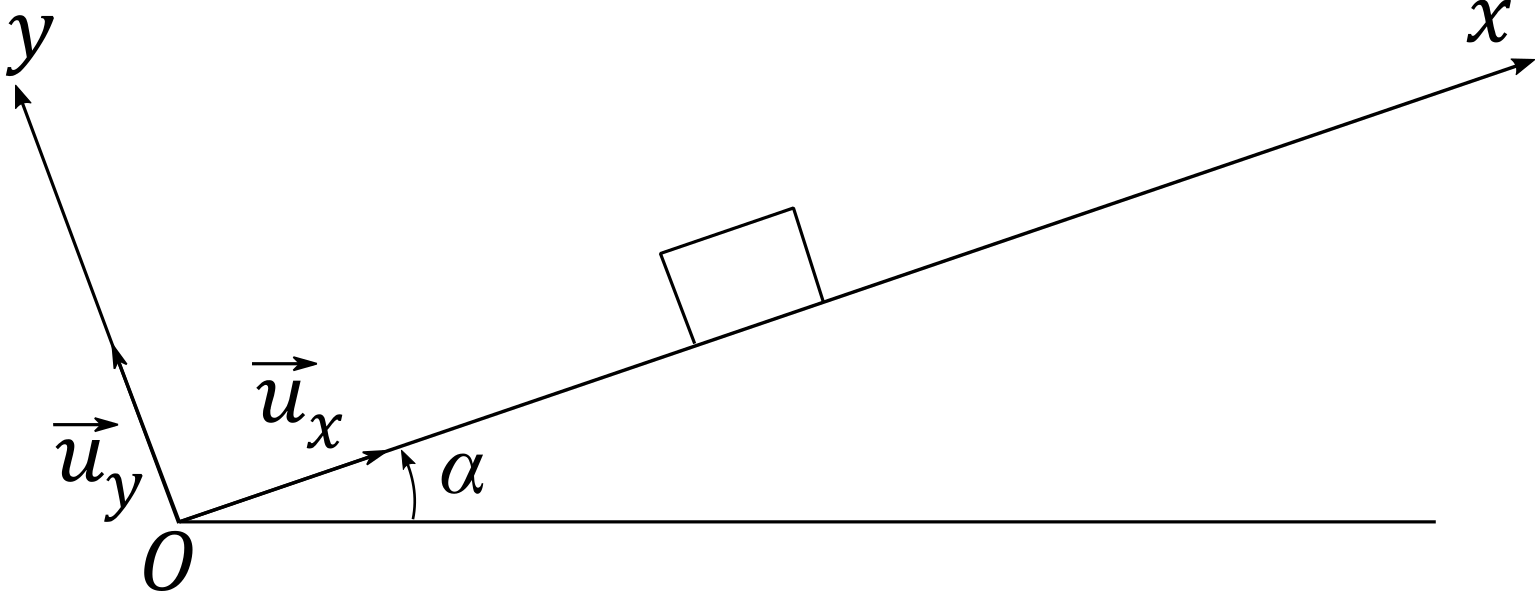
\includegraphics[width=\linewidth]{plan_incl-plain}
        \end{center}
    \end{minipage}
    \begin{enumerate}
        \item Établir l'équation horaire du mouvement de la brique lors de
            sa montée.
        \item Déterminer la date à laquelle la brique s'arrête, ainsi que la
            distance qu'elle aura parcourue.
    \end{enumerate}
\end{NCexem}
\begin{enumerate}[label=\sqenumi, resume]
    \item Étude du pendule simple~: mise en situation, équation différentielle,
        linéarisation, résolution \textit{via} PFD.
    \item Position d'équilibre d'un ressort vertical~: présenter le système,
        déterminer l'équation différentielle sur la position de la masse,
        déterminer la longueur d'équilibre, solution pour des conditions
        initiales données par l'interrogataire.
    \item Définir la puissance d'une force, son travail élémentaire, ainsi que
        son travail sur un chemin entre A et B.
    \item Énoncer et démontrer les théorèmes de la puissance cinétique et de
        l'énergie cinétique.
    \item Énoncer et démontrer les théorèmes de la puissance mécanique et de
        l'énergie mécanique.
    \item Retrouver les énergies potentielles de forces classiques (poids,
        rappel élastique, force newtonienne en $K/r^2$).
    \item Retrouver l'équation différentielle sur $\tt$ du pendule simple non
        amorti à l'aide~: soit du TPC, soit du TPM, au choix de
        l'interrogataire.
    \item Savoir discuter le mouvement d'une particule en comparant son profil
        d'énergie potentielle et son énergie mécanique~; état lié ou de
        diffusion. Expliquer l'obtention des positions d'équilibre et leur
        stabilité sur un graphique $\Ec_p(x)$. Traduire l'équilibre et sa
        stabilité en terme de conditions sur la dérivée première et seconde de
        l'énergie potentielle.
    \item Savoir réaliser l'approximation harmonique d'une cuvette de potentiel
        par développement limité. En déduire que tout système décrit par une
        énergie potentielle présentant un minimum local est assimilable à un
        oscillateur harmonique.
\end{enumerate}

\end{document}
